\chapter{From weak form to CUDA: one scalar problem, every stage}
\label{ch:c0}

\begin{keybox}
\textbf{Key idea.} Every solver in this course is the same assembly line:
a strong PDE becomes a weak form, the weak form becomes an element
residual and its Jacobian, quadrature turns those into numbers, a
local-to-global map scatters them into a sparse matrix, constraints and
boundary conditions are imposed, Newton linearizes, a linear solve runs
on the device, and the field updates. This chapter walks \emph{one} small
scalar problem down that line and names the \emph{exact} DiffSim file and
function at each stage --- so the phase-field bricks in the rest of the
course read as variations on a path you have already traced end to end.
Then you \textbf{do} the load-bearing step yourself: add a coefficient to
the weak form, derive its analytic Jacobian contribution, and watch a
regression test flip from red to green.
\end{keybox}

\section{The model}

We use the smallest problem that still has every ingredient of the
phase-field solvers: a \emph{nonlinear}, scalar, steady reaction--diffusion
equation on the unit square with Dirichlet data,
%
\begin{equation}
  -\grad^2 u + \alpha\,u^3 = f \quad\text{in } \Omega=(0,1)^2,
  \qquad u = g \ \text{on } \partial\Omega .
  \label{eq:c0strong}
\end{equation}
%
The Laplacian is the \emph{diffusion} (the same operator as the interface
term of Cahn--Hilliard); the cubic $\alpha u^3$ is a \emph{reaction} (a
stand-in for the nonlinear $f'(c)$ of the bulk free energy). One scalar
unknown per node keeps the bookkeeping visible; everything generalizes to
the mixed $(c,\mu)$ and multi-field blocks by carrying more degrees of
freedom per node.

\paragraph{Strong $\to$ weak (integration by parts).}
Multiply \eqref{eq:c0strong} by a test function $w$ that vanishes on the
Dirichlet boundary, integrate over $\Omega$, and move one derivative off
the Laplacian:
%
\begin{equation}
  -\intv w\,\grad^2 u \dV
  = \intv \grad w\cdot\grad u \dV - \int_{\partial\Omega} w\,(\grad u\cdot n)\dS .
\end{equation}
%
With $w=0$ on $\partial\Omega$ (strong Dirichlet) the surface term drops,
and the problem becomes: find $u$ such that for every admissible $w$,
%
\begin{equation}
  R(w;u) \;=\; \underbrace{\intv \grad w\cdot\grad u \dV}_{\text{diffusion}}
  \;+\; \underbrace{\alpha\intv w\,u^3 \dV}_{\text{reaction}}
  \;-\; \underbrace{\intv w\,f \dV}_{\text{load}} \;=\; 0 .
  \label{eq:c0weak}
\end{equation}

\paragraph{Element residual and its Jacobian.}
Expand $u_h=\sum_b N_b\,u_b$ and take $w=N_a$ (Galerkin). The residual
entry for node $a$ on element $e$ is \eqref{eq:c0weak} evaluated with
$w=N_a$. Because the reaction is nonlinear we solve by Newton, which needs
the \emph{tangent} $J=\dd{R}{u}$. Differentiating \eqref{eq:c0weak} in a
trial direction $N_b$,
%
\begin{equation}
  J_{ab} = \underbrace{\intv \grad N_a\cdot\grad N_b \dV}_{\text{stiffness (constant)}}
  \;+\; \underbrace{\alpha\intv N_a\,(3u^2)\,N_b \dV}_{\text{reaction Jacobian}} .
  \label{eq:c0jac}
\end{equation}
%
The derivative of $\alpha u^3$ is $3\alpha u^2$, so the reaction contributes
a \emph{$u$-weighted mass matrix} to the Jacobian. This second term is the
one you will add by hand in \S\ref{sec:c0hands}; the stiffness term is
$u$-independent and is assembled once.

\begin{keybox}
\textbf{Quadrature and the octree chain rule.} Every integral is a
Gauss sum $\int(\cdot)\dV=\sum_q(\cdot)|J|\,w_q$. On the octree's cube
elements the reference-to-physical map is a scaling by $h/2$, so
$|J|=(h/2)^{\text{dim}}$ and physical gradients are reference gradients
times $\code{dscale}=2/h$. The tables $N_a(x_q)$, $\grad N_a(x_q)$ and
$w_q$ come from \file{mesh/basis.py} (\code{basis\_tables},
\code{gauss\_1d}); inside a kernel they are read through the
\file{assembly/femelm.py} accessors \code{fe\_N}, \code{fe\_dN\_s},
\code{fe\_detJxW\_s}. The tutorial's readable NumPy assembly uses exactly
these tables --- and a test proves its stiffness matrix equals the
production Warp-kernel assembly to the last bit.
\end{keybox}

\section{The pipeline, stage by stage}

Figure~\ref{fig:c0pipeline} is the map: the left column is the stage, the
right column is the DiffSim file and function that owns it. The tutorial
file \file{scalar\_reaction.py} implements the whole path in transparent
NumPy/SciPy (one function per stage, each annotated with its production
counterpart), so you can read a stage here, then open the one line of code
that does it, then open the production kernel it mirrors.

\begin{figure}[h]\centering
  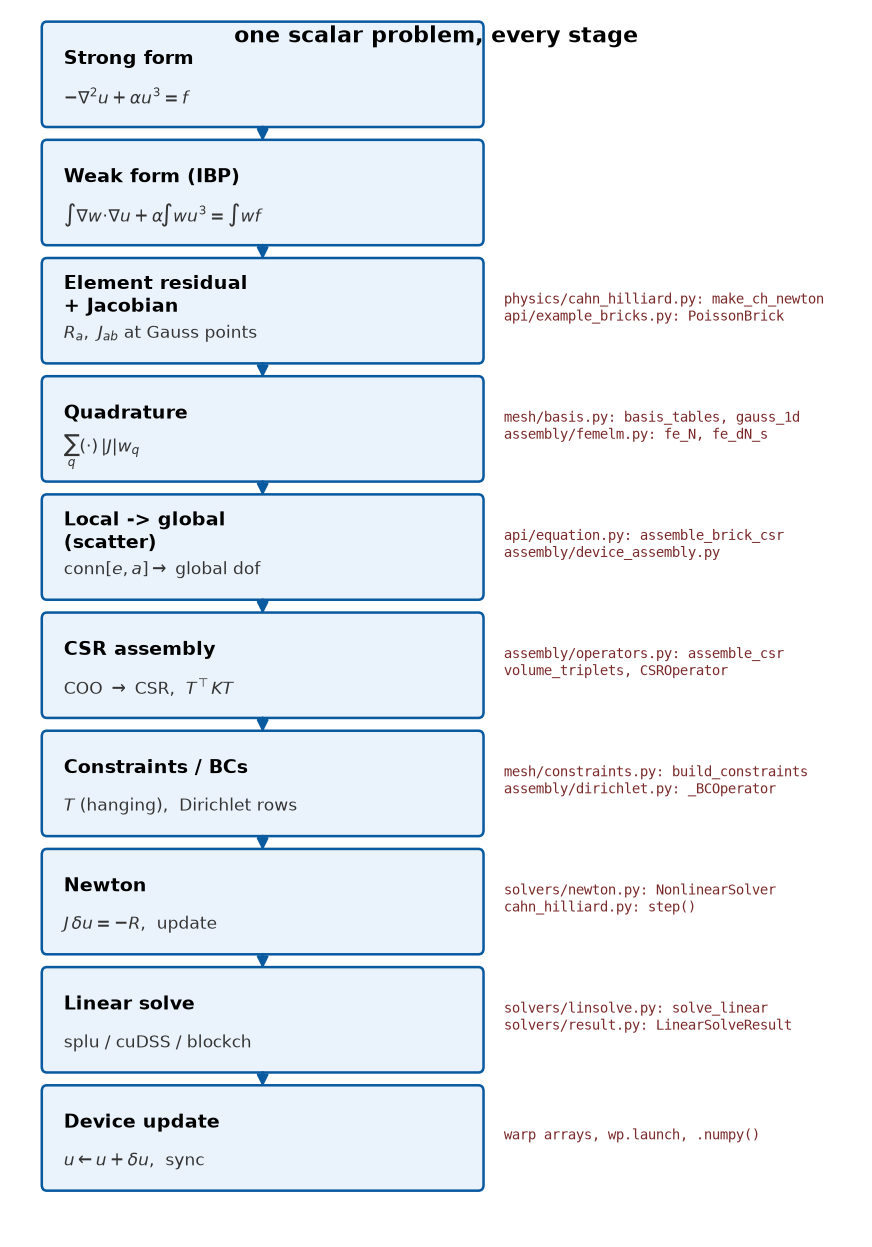
\includegraphics[height=0.92\textheight]{figures/c0_pipeline.png}
  \caption{The weak-form-to-CUDA pipeline for one scalar problem. Each
    stage (left) maps to the exact DiffSim source (right). The tutorial's
    \file{scalar\_reaction.py} walks the whole path in readable NumPy; the
    phase-field bricks (\file{physics/cahn\_hilliard.py} and siblings) are
    the same path with more fields per node and the arithmetic in Warp
    kernels.}
  \label{fig:c0pipeline}
\end{figure}

\begin{enumerate}[nosep]
  \item \textbf{Mesh + basis.}
        \code{build\_uniform} (\file{octree/build.py}) $\to$
        \code{build\_mesh} (\file{mesh/nodes.py}) $\to$
        \code{build\_constraints} (\file{mesh/constraints.py}) $\to$
        \code{basis\_tables} (\file{mesh/basis.py}) $\to$
        \code{DeviceMesh.from\_mesh} (\file{assembly/operators.py}). The
        \code{DeviceMesh} holds the per-degree connectivity, the basis
        tables, and the constraint matrix $T$, all as device arrays.
  \item \textbf{Element residual + Jacobian.} The physics of one
        integration point. The production phase-field kernel is
        \code{make\_ch\_newton} (\file{physics/cahn\_hilliard.py}); the
        linear model brick is \code{PoissonBrick}
        (\file{api/example\_bricks.py}), whose \code{Integrands\_Ae}/
        \code{Integrands\_be} are the annotated ``write the weak form, get
        the assembly'' API.
  \item \textbf{Quadrature.} \code{basis\_tables} / \code{gauss\_points}
        (\file{physics/poisson.py}) supply $x_q$, $N$, $\grad N$, $w_q$.
  \item \textbf{Local $\to$ global (scatter).} The element block
        $\mathrm{conn}[e,a]\!\to$ global dof; \code{assemble\_brick\_csr}
        (\file{api/equation.py}) or the device scatter kernels of
        \file{assembly/device\_assembly.py}.
  \item \textbf{CSR assembly.} COO triplets $\to$ CSR, then the
        constrained $T^{\!\top}\!K\,T$; \code{assemble\_csr} /
        \code{volume\_triplets} / \code{CSROperator}
        (\file{assembly/operators.py}).
  \item \textbf{Constraints / BCs.} Hanging-node interpolation is the
        matrix $T$ from \code{build\_constraints}; strong Dirichlet is row
        replacement (\code{\_BCOperator}, \file{assembly/dirichlet.py}; and
        the CH stepper's own row replacement in \code{step}).
  \item \textbf{Newton.} \code{NonlinearSolver} (\file{solvers/newton.py})
        or the monolithic loop in \code{CahnHilliardStepper.step}: assemble
        $J,R$; solve $J\,\delta u=-R$; line-search; update.
  \item \textbf{Linear solve.} \code{solve\_linear}
        (\file{solvers/linsolve.py}) dispatches \code{splu} (host direct),
        \code{cudss} (GPU direct), \code{blockch} (the mixed-CH Schur
        preconditioner), returning a \code{LinearSolveResult}
        (\file{solvers/result.py}).
  \item \textbf{Device update.} The solution vector updates the field
        state; host/device transfers are the \code{wp.array(\dots)} uploads
        and \code{.numpy()} pulls around \code{wp.launch}.
\end{enumerate}

\begin{keybox}
\textbf{Where the tutorial meets production.} For a \emph{uniform} box
there are no hanging nodes, so the constraint matrix $T$ is the identity
and the free-node system is just the node system --- which is why
\file{scalar\_reaction.py} can impose Dirichlet data by row replacement and
skip $T$. The chapter's cross-check test asserts that its hand-assembled
stiffness equals \code{assemble\_brick\_csr(dm, PoissonBrick())} (the
production Warp kernel through $T^{\!\top}\!K\,T$) to
$\CzeroStiffDiff$ --- the transparent NumPy \emph{is} the device math.
\end{keybox}

\section{Hands-on: add a coefficient and its analytic Jacobian}
\label{sec:c0hands}

This is the exercise. The starter file \file{scalar\_reaction\_starter.py}
already has the reaction term $\alpha u^3$ in the \emph{residual}, so it
solves the right PDE --- but its \emph{Jacobian} is missing the reaction
contribution \eqref{eq:c0jac}. A Newton solve with a wrong Jacobian may
still limp to an answer, so a convergence check alone would not catch the
bug. The sharp, hardware-independent test is a \textbf{derivative check}:
the analytic Jacobian must match a finite difference of the residual,
%
\begin{equation}
  \frac{\big\|\,J(u)\,v \;-\; \big(R(u+\varepsilon v)-R(u)\big)/\varepsilon\,\big\|}
       {\big\|\big(R(u+\varepsilon v)-R(u)\big)/\varepsilon\big\|}
  \;\ll\; 1 .
  \label{eq:c0fd}
\end{equation}

\begin{runbox}
\textbf{Do it (red $\to$ green).}
\begin{lstlisting}
cd computational/00_weak_form_to_cuda
# 1. RED: the starter's Jacobian omits the reaction term
RD_MODULE=scalar_reaction_starter pytest -q test_reaction_jacobian.py
# 2. Add the analytic reaction Jacobian to jacobian() in the module
#    you are editing (the completed reference is scalar_reaction.py):
#       Ke = prob._Ke + reaction_jacobian_elem(prob, gp_value(prob, u))
# 3. GREEN:
pytest -q test_reaction_jacobian.py
\end{lstlisting}
\end{runbox}

With the reaction Jacobian \emph{missing}, \eqref{eq:c0fd} is
$\CzeroJacStarter$ --- the test fails. With the analytic term
$3\alpha u^2$ \emph{added}, it is $\CzeroJacOk$ (finite-difference
truncation only) --- the test passes. The same edit restores Newton's
\emph{quadratic} convergence (Fig.~\ref{fig:c0verify}, right): the residual
norm is squared each step once the tangent is exact.

\begin{keybox}
\textbf{Why a derivative test, not just ``it converged''.} A missing or
wrong Jacobian term is the single most common bug when adding physics to an
implicit solver, and it hides well: the residual (the equation you solve)
can be perfectly correct while the tangent (how you get there) is wrong, so
the run still lands near an answer, just slowly or fragilely. The
finite-difference check in \eqref{eq:c0fd} tests the tangent \emph{directly}
and deterministically --- it is the same check the differentiable track and
any new-term workflow (residual $\to$ analytic Jacobian $\to$ derivative
test) must pass before an order or a gradient is trusted.
\end{keybox}

\section{Run it: verify the whole pipeline}

\begin{runbox}
\textbf{Run it.}
\begin{lstlisting}
cd computational/00_weak_form_to_cuda
python run.py --config configs/c0.yaml --device cpu --solver splu \
    --mode reference --output outputs/c0 --overwrite
python gen_figures.py --run-dir outputs/c0
\end{lstlisting}
The harness runs the manufactured-solution convergence study ($p{=}1$ and
$p{=}2$), the Newton-convergence trace, the analytic-Jacobian check (against
both the completed and the starter modules), and the production-kernel
cross-check; it writes \file{results.json}, checks it against
\file{baseline.yaml} (tolerances, not bit-identity), and records provenance
in \file{metadata.json}. \code{gen\_figures.py} renders the figures and
\file{numbers/c0.tex} from the saved run.
\end{runbox}

\paragraph{What you should see.} We verify the assembly is correct with the
\emph{method of manufactured solutions}: pick $u^\star=\sin(\pi x)\sin(\pi
y)$ (zero on the boundary), feed the source
$f=2\pi^2 u^\star+\alpha (u^\star)^3$ that makes it exact, and measure the
$L^2$ error under mesh refinement. Degree-$p$ elements converge at $h^{p+1}$
--- the single most diagnostic correctness check for a discretization. The
measured orders are $\CzeroPoneOrder$ ($p{=}1$) and $\CzeroPtwoOrder$
($p{=}2$), on the predicted lines (Fig.~\ref{fig:c0verify}, left).

\begin{figure}[h]\centering
  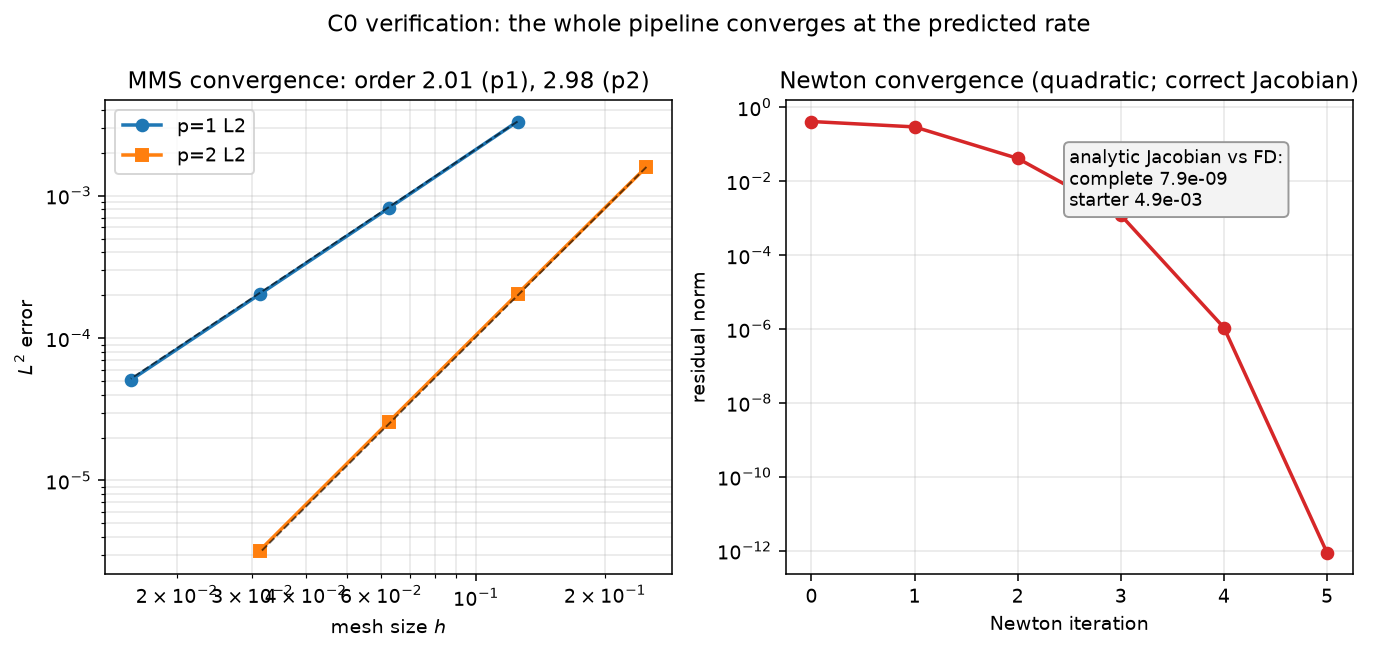
\includegraphics[width=\linewidth]{figures/c0_convergence.png}
  \caption{Verification of the whole pipeline. \emph{Left:} manufactured-
    solution $L^2$ error falls at the predicted $h^{p+1}$ rate (order
    $\CzeroPoneOrder$ for $p{=}1$, $\CzeroPtwoOrder$ for $p{=}2$), proof
    every stage is assembled correctly. \emph{Right:} with the correct
    analytic Jacobian, Newton converges quadratically (residual
    $\CzeroNewtonResZero\to\CzeroNewtonResFinal$ in $\CzeroNewtonIters$
    iterations); the inset contrasts the analytic-vs-finite-difference
    Jacobian error for the completed brick and the hands-on starter.}
  \label{fig:c0verify}
\end{figure}

\begin{keybox}
\textbf{Measured self-check} (reference mode, \code{splu}; reproduced within
\file{baseline.yaml} tolerances, not bit-for-bit).
\begin{center}\small
\begin{tabular}{lcc}
\toprule
 & $p=1$ & $p=2$ \\
\midrule
$L^2$ error: coarse $\to$ fine & \CzeroPoneErrCoarse\ $\to$ \CzeroPoneErrFine
                               & \CzeroPtwoErrCoarse\ $\to$ \CzeroPtwoErrFine \\
observed order (expect $p{+}1$) & \CzeroPoneOrder\ ($2$) & \CzeroPtwoOrder\ ($3$) \\
\midrule
\multicolumn{3}{l}{Newton (level 5): residual \CzeroNewtonResZero\ $\to$ \CzeroNewtonResFinal\ in \CzeroNewtonIters\ iterations} \\
\multicolumn{3}{l}{analytic Jacobian vs FD: \CzeroJacOk\ (complete) \emph{vs} \CzeroJacStarter\ (starter, reaction Jac missing)} \\
\multicolumn{3}{l}{transparent stiffness vs production kernel: \CzeroStiffDiff} \\
\bottomrule
\end{tabular}
\end{center}
\end{keybox}

\section{Code walk-through}

\file{scalar\_reaction.py} is organized one function per pipeline stage.

\paragraph{1. Mesh + tables (the real path).}
\begin{lstlisting}
tree = build_uniform(level, dim=2)          # octree/build.py
mesh = build_mesh(tree, p)                   # mesh/nodes.py
cons = build_constraints(mesh)               # mesh/constraints.py
dm   = DeviceMesh.from_mesh(mesh, cons, basis_tables(p, 2), device)
\end{lstlisting}
The same four calls every tutorial makes; \code{basis\_tables} gives $N$,
$\grad N$ (reference) and $w_q$, and the octree factors $\code{dscale}=2/h$,
$|J|=(h/2)^{\dim}$ convert to physical space.

\paragraph{2. Element residual + Jacobian (quadrature by \code{einsum}).}
\begin{lstlisting}
def reaction_jacobian_elem(prob, uq):        # the hands-on term
    wq = 3.0 * prob.alpha * uq**2            # d/du (alpha u^3)
    return einsum("qa,eq,qb,q->eab", N, wq, N, detJxW)  # INT N_a (3 a u^2) N_b
\end{lstlisting}
The \code{einsum} \emph{is} the Gauss sum of \eqref{eq:c0jac}; the diffusion
stiffness is the same pattern with $\grad N_a\cdot\grad N_b$.

\paragraph{3. Local-to-global + Dirichlet, then the real solve.}
\begin{lstlisting}
J = coo_matrix((Ke.ravel(), (rows, cols))).tocsr()   # scatter -> CSR
J.rows[i] = [i]; J.data[i] = [1.0]                   # Dirichlet row = I
du = solve_linear(J, -R, solver="splu")              # solvers/linsolve.py
\end{lstlisting}
\code{rows}/\code{cols} are the connectivity outer-product --- the exact
triplet pattern \code{assemble\_brick\_csr} builds --- and the linear solve
is the production dispatcher, so swapping \code{"splu"} for \code{"cudss"}
runs the same Newton step on the GPU.

\section{Explore on your own}

\question{Change the reaction to $\alpha u^5$. Write its residual and the
analytic Jacobian weight ($5\alpha u^4$), update both, and confirm the
derivative check \eqref{eq:c0fd} passes and Newton stays quadratic. What
happens to the convergence if you update the residual but \emph{not} the
Jacobian?}

\question{Switch the linear solve from \code{splu} to \code{cudss}
(\code{--solver cudss}, GPU). The Newton iterates and the $L^2$ error should
be identical to solver tolerance --- verify that the \emph{discretization}
answer does not depend on the \emph{linear-algebra} backend.}

\question{Make the reaction coefficient a field, $\alpha(x)$. Which pipeline
stage changes --- the residual, the Jacobian, the assembly, or the solve?
(Hint: only the integrand; the scatter and solve are untouched. This is why
the brick API asks you for one integration point.)}

\question{Push the $p{=}1$ study to level 7. Does the order stay $2$, or does
round-off floor the error? Predict the level from the coarse-grid error and
machine epsilon, then confirm.}

\question{Read \code{make\_ch\_newton} in \file{physics/cahn\_hilliard.py}
and match its four $2\times2$ Jacobian blocks
($\dd{R_c}{c},\dd{R_c}{\mu},\dd{R_\mu}{c},\dd{R_\mu}{\mu}$) to the single
scalar $J_{ab}$ of this chapter. Which block is the analogue of the reaction
Jacobian you added here?}

% ====================================================================
